
\documentclass[
	% -- opções da classe memoir --
	12pt,				% tamanho da fonte
	% openright,			% capítulos começam em pág ímpar (insere página vazia caso preciso)
    oneside,			% para impressão somente frente. Oposto a twoside (frente e verso)
	a4paper,			% tamanho do papel. 
	% -- opções da classe abntex2 --
	%chapter=TITLE,		% títulos de capítulos convertidos em letras maiúsculas
	%section=TITLE,		% títulos de seções convertidos em letras maiúsculas
	%subsection=TITLE,	% títulos de subseções convertidos em letras maiúsculas
	%subsubsection=TITLE,% títulos de subsubseções convertidos em letras maiúsculas
	% -- opções do pacote babel --
	english,			% idioma adicional para hifenização
	french,				% idioma adicional para hifenização
	spanish,			% idioma adicional para hifenização
	brazil,				% o último idioma é o principal do documento
	]{abntex2}


% ---
% PACOTES
% ---

% ---
% Pacotes fundamentais 
% ---
\usepackage{cmap}				% Mapear caracteres especiais no PDF
\usepackage{lmodern}			% Usa a fonte Latin Modern
\usepackage[T1]{fontenc}		% Selecao de codigos de fonte.
\usepackage[utf8]{inputenc}		% Codificacao do documento (conversão automática dos acentos)
\usepackage{indentfirst}		% Indenta o primeiro parágrafo de cada seção.
\usepackage{color}				% Controle das cores
\usepackage{graphicx}			% Inclusão de gráficos
% ---

% ---
% Pacotes adicionais, usados no anexo do modelo de folha de identificação
% ---
\usepackage{multicol}
\usepackage{multirow}
% ---
	
% ---
% Pacotes adicionais, usados apenas no âmbito do Modelo Canônico do abnteX2
% ---
\usepackage{lipsum}				% para geração de dummy text
% ---

% ---
% Pacotes de citações
% ---
\usepackage[brazilian,hyperpageref]{backref}	 % Paginas com as citações na bibl
\usepackage[alf]{abntex2cite}	% Citações padrão ABNT

% --- 
% CONFIGURAÇÕES DE PACOTES
% --- 

% ---
% Configurações do pacote backref
% Usado sem a opção hyperpageref de backref
\renewcommand{\backrefpagesname}{Citado na(s) página(s):~}
% Texto padrão antes do número das páginas
\renewcommand{\backref}{}
% Define os textos da citação
\renewcommand*{\backrefalt}[4]{
	\ifcase #1 %
		Nenhuma citação no texto.%
	\or
		Citado na página #2.%
	\else
		Citado #1 vezes nas páginas #2.%
	\fi}%
% ---

% ---
% Informações de dados para CAPA e FOLHA DE ROSTO
% ---
\titulo{Projeto Integrador}
\autor{Náthaly do Amaral Verzas}
\local{Brasil}
\data{Setembro de 2017}
\instituicao{%
  Serviço Nacional de Aprendizagem Comercial -SENAC
  \par
  Técnico em Informática
  \par
  Website Contabilidade - Real Céllos}
\tipotrabalho{Relatório técnico}
% O preambulo deve conter o tipo do trabalho, o objetivo, 
% o nome da instituição e a área de concentração 
\preambulo{Relatório Técnico do website criado para o projeto integrador, apresentado ao SENAC como requisito de obtenção do certificado do curso técnico em informática. \LaTeX.}
% ---

% ---
% Configurações de aparência do PDF final

% alterando o aspecto da cor azul
\definecolor{blue}{RGB}{41,5,195}

% informações do PDF
\makeatletter
\hypersetup{
     	%pagebackref=true,
		pdftitle={\@title}, 
		pdfauthor={\@author},
    	pdfsubject={\imprimirpreambulo},
	    pdfcreator={LaTeX with abnTeX2},
		pdfkeywords={abnt}{latex}{abntex}{abntex2}{relatório técnico}, 
		colorlinks=true,       		% false: boxed links; true: colored links
    	linkcolor=blue,          	% color of internal links
    	citecolor=blue,        		% color of links to bibliography
    	filecolor=magenta,      		% color of file links
		urlcolor=blue,
		bookmarksdepth=4
}
\makeatother
% --- 

% --- 
% Espaçamentos entre linhas e parágrafos 
% --- 

% O tamanho do parágrafo é dado por:
\setlength{\parindent}{1.3cm}

% Controle do espaçamento entre um parágrafo e outro:
\setlength{\parskip}{0.2cm}  % tente também \onelineskip

% ---
% compila o indice
% ---
\makeindex
% ---

% ----
% Início do documento
% ----
\begin{document}

% Retira espaço extra obsoleto entre as frases.
\frenchspacing 

% ----------------------------------------------------------
% ELEMENTOS PRÉ-TEXTUAIS
% ----------------------------------------------------------
% \pretextual

% ---
% Capa
% ---
\imprimircapa
% ---

--
% RESUMO
% ---

% resumo na língua vernácula (obrigatório)
\begin{resumo} %% AQUI COMEÇA A PÁGINA DE RESUMO
 Este documento tem o objetivo de apresentar e especificar toda a funcionalidade do website criado para o projeto. Como métodos de implementação, justificativa da realização do projeto.

 \vspace{\onelineskip}
    
 \noindent
 \textbf{Palavras-chaves}: Desenvolvedor Web. Site de Contabilidade.
\end{resumo} %AQUI TERMINA A PÁGINA DE RESUMO
% ---

% ---
% inserir lista de ilustrações
% ---


% ---

% ---
% inserir o sumario
% ---

\tableofcontents*

% ---

% ----------------------------------------------------------
% ELEMENTOS TEXTUAIS  (necessário para incluir número nas páginas)
% ----------------------------------------------------------
\textual


% ----------------------------------------------------------
% Introdução
% ----------------------------------------------------------
\chapter{Introdução} %% NOVO CAPÍTULO (REPARE QUE ELE AUTOMATICAMENTE JÁ COLOCA O NÚMERO DO CAPÍTULO E JÁ ADICIONA NO SUMÁRIO)



Ter uma página na internet se tornou indispensável para empresas de todos os tamanhos: grande, médio ou pequeno porte. Esta ferramenta possibilita comunicação junto ao seu cliente sobre os seus produtos e serviços, apresentando seus diferenciais. Mas não basta ter um site "bonitinho" e esperar que chova clientes! Pelo contrário, ter um site na internet é apenas o primeiro passo para a empresa que está "engatinhando" no mundo virtual, é o começo de muito trabalho para que essa ferramenta seja utilizada de forma inteligente, que possa corresponder positivamente ao tempo e dinheiro investidos.

Não é mais possível pedir ao "sobrinho de seu amigo que entende de computador" para fazer um site para sua empresa. Um site é a imagem de sua empresa na internet e, assim como você não compareceria à uma reunião de bermuda e camiseta, seu site deve ser o mais bem elaborado possível. 

Através destes critérios foi escolhido desenvolver um website para empresa de Contabilidade Real Céllos proposta no projeto. 

\chapter{Proposta}

De acordo com os blocos no curso o projeto iria tendo propostas diferentes voltada ao conteúdo do bloco atual, sempre é solicito uma empresa fictícia com proprietário Delson. Neste bloco final a empresa de Delson agora já está no mundo digital, com toda sua estrutura funcionando em rede, porém
deseja-se expandir o seu negócio e resolve que sua empresa precisa ter sua própria marca na
era digital, para isso ele propôs 2 opções de negócio:\\
\\1. Criação de um software para a empresa;\\
\\2. Criação de um Website para a empresa;\\

Delson pesquisou e encontrou vários técnicos em informática que estavam aptos para esta tarefa,
resolveu então pedir para que cada um escolhesse uma das opções e entregasse o projeto final para que
ele escolhesse qual ele usaria em sua empresa, sendo os técnicos ou alunos. O projeto escolhido foi um website para um escritório de contabilidade, com a marca Real Céllos.


\chapter{Design}

\subsection{Logo}

Uma logo é a representação gráfica do nome da empresa ou marca, que determina a sua identidade visual e tem como objetivo facilitar o seu reconhecimento. Uma logomarca dá sentido à marca em questão, identificando-a e definindo-a no tempo e no espaço, como definido o nome Real Céllos foi criado esta logo marca para a empresa:\\

\begin{figure}[!h]
\center

\includegraphics[width=0.5\textwidth]{logo.png}
\caption{Logo Marca}
\end{figure}

\subsection{Modelo Layout}

 É o design da página web. Ele é composto de todos os elementos que são mostrados quando você acessa um site - o arranjo, as formas, as cores, tipografias, etc. O escolhido é responsivo, ou também conhecido como site flexível é quando o site automaticamente se encaixa no dispositivo do usuário (PC, celular, tablet, etc). Segue o exemplo:\\
 
 \begin{figure}[!h]
\center
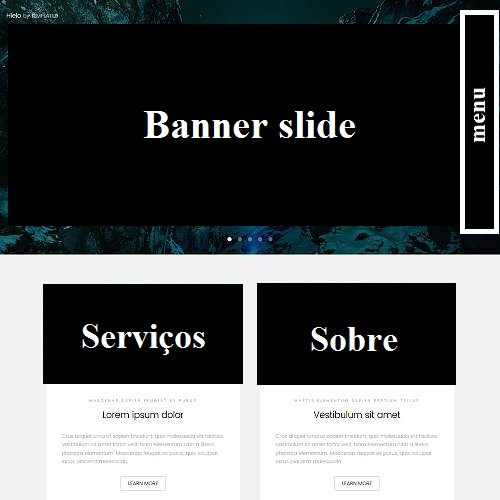
\includegraphics[width=0.9\textwidth]{hielo.jpg}
\caption{Layout}
\end{figure}

\chapter{Estrutura do site}

O site é estruturado por cabeçalho, menu lateral e rodapé, contém uma página inicial, página de informações sobre a empresa, página de notícias, página de serviços, página de contato e um painel de administrador de conteúdo.

Para implementação foi usado o software Adobe Dreamweaver CS6, para programação em linguagem de interpretação html, css, linguagem de programação php e scripts de javascript. 

O site possui um painel administrador implementado com banco de dados, onde as tabelas são ligadas a variáveis no código php, isto evita que o usuário tenha que acessar diretamente no código fonte para fazer alterações. O painel administrativo é o local onde é realizado o gerenciamento do site atraves de uma interface. O acesso é feito linkado a página index(Pagina inicial do site), como todo painel administrador ele exige uma autenticação. 

Seu acesso é por meio do navegador de internet, no campo “endereço” ou URL, localizado na parte superior do navegador, deve-se informar o endereço de acesso ao painel, adicionando ao final a palavra “index.php/admin” \\(http://www.dominiodaloja.com.br/admin/).

\chapter{Página Inicial}

A página inicial é composta por slides automáticos de apresentação do site, informações de serviços. Há pequenos box (caixas).

Separadas por 3 <div>:

\begin{itemize}
	\item{Cabeçalho: Slides de banners feito em Javascript, <div> de cabeçalho com CSS personalizada para o cabeçalho.}
	\item{Corpo: Corpo é uma <div> divididas em duas colunas. A primeira tem 1 caixa (box) que é uma breve descrição da página de serviços, composta por um botão(button), ao sobrepor o cursor do mouse em cima o javascript de opacidade é ativado, dando a impressão que está sendo destacado esse botão identificado como "SAIBA MAIS", tanto para a segunda coluna possui botão de "SAIBA MAIS", ao clicar no botão de serviços o site redireciona o usuário para a página de serviços, caso vá na segunda coluna tem 2 caixas, a primeira é "Sobre" a empresa e a segunda de noticias. \\ O corpo ainda possui uma <div> de galeria que através do CSS esta div de galeria permite ter 2 colunas com varias caixas de link de imagens mostradas do escritório.}
	\item{Rodapé: é uma <div> com personalização de CSS único, pois este rodapé é igual em todas as páginas, nele possui informações de direitos autorais do desenvolvedor e ícones linkados às redes sociais da empresa.}
	
	\item{Menu lateral-direito: Este menu permite ao usuário visualizar as páginas disponíveis para acesso. São elas: 
	
	\begin{itemize}
			
	\item{Home (Página principal)}
	\item{Sobre (Página de informações sobre a empresa)}
	\item{Serviços (Página descrevendo, e informando todos os serviços oferecidos pela empresa)} 		    \item{Notícias (Página que oferece ao usuário estar sempre atualizado com as últimas novidades da bolsa de valores)}
	
	\end{itemize}
	
	Estas opções de páginas ficam implícitas para o usuário em todas as páginas, para exibir o usuário deve clicar no "MENU" é ativado um javascript de animação.
}
\end{itemize}

\chapter{Página: Sobre Empresa}

A página Quem Somos com texto sobre a empresa aproxima seu negócio do cliente. Aqui diz o que sua empresa faz e qual o objetivo dela.

\begin{itemize}
	\item{Cabeçalho: Possui uma <div> personalizada diferente do cabeçalho da página principal, pois esta apenas tem o CSS simples com background preto, está é estabelecida para as demais páginas pois possui o titulo de identificação do que se trata nesta página.}
	\item{Corpo: Conteúdo de histórico da empresa em uma <div> personalizada como corpo de página de informações, este mesmo CSS irá ser usado para as demais páginas.}
	\item{Rodapé: é uma <div> com personalização de CSS único, pois este rodapé é igual em todas as páginas, nele possui informações de direitos autorais do desenvolvedor e ícones linkados às redes sociais da empresa.}
	
	\item{Menu lateral-direito: Este menu permite ao usuário visualizar as páginas disponíveis para acesso. São elas: 
	
	\begin{itemize}
			
	\item{Home (Página principal)}
	\item{Sobre (Página de informações sobre a empresa)}
	\item{Serviços (Página descrevendo, e informando todos os serviços oferecidos pela empresa)} 		    \item{Notícias (Página que oferece ao usuário estar sempre atualizado com as últimas novidades da bolsa de valores)}
	
	\end{itemize}
	
	Estas opções de páginas ficam implícitas para o usuário em todas as páginas, para exibir o usuário deve clicar no "MENU" é ativado um javascript de animação.
}
\end{itemize}

\chapter{Página de Noticias}

A página de noticias permite que o usuário encontre, em uma mesma página, vídeos, notícias, entretenimento e conteúdos relacionado ao site.


\begin{itemize}
	\item{Cabeçalho: Possui uma <div> personalizada diferente do cabeçalho da página principal, pois esta apenas tem o CSS simples com background preto, está é estabelecida para as demais páginas pois possui o titulo de identificação do que se trata nesta página.}
	\item{Corpo: Contém o as noticias publicadas no site.}
	\item{Rodapé: é uma <div> com personalização de CSS único, pois este rodapé é igual em todas as páginas, nele possui informações de direitos autorais do desenvolvedor e ícones linkados às redes sociais da empresa.}
	
	\item{Menu lateral-direito: Este menu permite ao usuário visualizar as páginas disponíveis para acesso. São elas: 
	
	\begin{itemize}
			
	\item{Home (Página principal)}
	\item{Sobre (Página de informações sobre a empresa)}
	\item{Serviços (Página descrevendo, e informando todos os serviços oferecidos pela empresa)} 		    \item{Notícias (Página que oferece ao usuário estar sempre atualizado com as últimas novidades da bolsa de valores)}
	
	\end{itemize}
	
	Estas opções de páginas ficam implícitas para o usuário em todas as páginas, para exibir o usuário deve clicar no "MENU" é ativado um javascript de animação.
}
\end{itemize}

\chapter{Página de Serviços}

Na página Serviços deixa claro tudo o que oferece. É importante criar uma página desse para que os serviços possam ser apresentados das mais diversas áreas, como: Assessoria Fiscal, Assessoria Contábil, Assessoria Trabalhista, Encerramentos de Empresas, Imposto de Renda Pessoa Física. 

\begin{itemize}
	\item{Cabeçalho: Possui uma <div> personalizada diferente do cabeçalho da página principal, pois esta apenas tem o CSS simples com background preto, está é estabelecida para as demais páginas pois possui o titulo de identificação do que se trata nesta página.}
	\item{Corpo: Contém todos os serviços da empresa com sua descrição.}
	\item{Rodapé: é uma <div> com personalização de CSS único, pois este rodapé é igual em todas as páginas, nele possui informações de direitos autorais do desenvolvedor e ícones linkados às redes sociais da empresa.}
	
	\item{Menu lateral-direito: Este menu permite ao usuário visualizar as páginas disponíveis para acesso. São elas: 
	
	\begin{itemize}
			
	\item{Home (Página principal)}
	\item{Sobre (Página de informações sobre a empresa)}
	\item{Serviços (Página descrevendo, e informando todos os serviços oferecidos pela empresa)} 		    \item{Notícias (Página que oferece ao usuário estar sempre atualizado com as últimas novidades da bolsa de valores)}
	
	\end{itemize}
	
	Estas opções de páginas ficam implícitas para o usuário em todas as páginas, para exibir o usuário deve clicar no "MENU" é ativado um javascript de animação.
}
\end{itemize}

\chapter{Página de contato}

Um formulário de contato em seu site facilita a comunicação de seus clientes e pessoas que têm interesse em seu negócio. Sua implementação é bastante simples feita em php e html.

\begin{itemize}
	\item{Cabeçalho: Possui uma <div> personalizada diferente do cabeçalho da página principal, pois esta apenas tem o CSS simples com background preto, está é estabelecida para as demais páginas pois possui o titulo de identificação do que se trata nesta página.}
	\item{Corpo: Formulário de contato, este feito em HTML, está contido em um <form>, pois o form dá as opções de entrada de dados, e botões de ações que podem ser usados para limpar as informações do formilário ou enviar. O envio acontece por um clica em um botão que tem uma ação sobre o form, como métodos POST, que pega todos os valores dentro do campo do formulário e através do php executa a parte lógica de enviar esses valores para o email da empresa.}
	\item{Rodapé: é uma <div> com personalização de CSS único, pois este rodapé é igual em todas as páginas, nele possui informações de direitos autorais do desenvolvedor e ícones linkados às redes sociais da empresa.}
	
	\item{Menu lateral-direito: Este menu permite ao usuário visualizar as páginas disponíveis para acesso. São elas: 
	
	\begin{itemize}
			
	\item{Home (Página principal)}
	\item{Sobre (Página de informações sobre a empresa)}
	\item{Serviços (Página descrevendo, e informando todos os serviços oferecidos pela empresa)} 		    \item{Notícias (Página que oferece ao usuário estar sempre atualizado com as últimas novidades da bolsa de valores)}
	
	\end{itemize}
	
	Estas opções de páginas ficam implícitas para o usuário em todas as páginas, para exibir o usuário deve clicar no "MENU" é ativado um javascript de animação.
}
\end{itemize}

\chapter{Banco de Dados}

O site tem um sistema de banco de dados, isto permite a criação do painel administrador de conteúdo. O phpMyAdmin é um sistema de gerenciamento de bases de dados online, ou seja, você utiliza seu navegador para criar, apagar e editar tabelas e bancos de dados no servidor MySQL. 

\subsection{Painel Administrador}

O gerenciador de conteúdo é uma ferramenta que permite manusear o conteúdo do site sem a necessidade de fazer alteração no conteúdo de serviços, noticias, banco de imagens e links. Com ele podemos adicionar, editar ou excluir conteúdo (fotos, vídeos, documentos, etc.), independente do dispositivo ou sistema operacional que você esteja utilizando.

Feito em php e com conexão no banco de dados. O banco funciona com as variáveis que recebem cada campo que deseja ser editado através do painel, isto é as páginas que desejam ter gerenciamento de conteúdo tem php para fazer a parte lógica do site que liga os valores ao banco de dados. 

O banco de dados é configurado pelo dominio oferecido. Para o painel funcionar tempos uma página de Login, Dashboard(Painel), Autenticação.

\begin{itemize}
	\item{Login: é uma página em php que contem as div de cabeçalho, corpo, rodapé e menu lateral-direito. O login tem um form para inserir as informações de usuário e senha. Há um botão para submeter essas informações para a página que faz autenticação.}
	\item{Autenticação: Serve como componente principal de segurança e inicia a conexão com o banco, está é ativada quando o usuário submete as informações de usuário e senha pelo painel de login, ela então executa o comando de banco de dados SELECT * FROM, para selecionar o id, usuario e senha preenchidas na tabela usuários no banco de dados, quando ele pega estes valores ele compara através de condicionais de comparação em php IF e ELSE, se o usuário é autenticado a página redericiona para a Dashboard que é o painel de editar, excluir, atualizar e adicionar conteúdo.}
	\item{Dashboard: Está página contem um layout como um banco de dados, nela é permitido alterar a logo da empresa, alterar as imagens do slide-banner, os serviços oferecidos da empresa, as noticias, e os links da redes sociais citadas no rodapé. Em cada tabela possui os botões de editar, excluir e ver.}
\end{itemize} 

\chapter[Conclusão]{Conclusão}

Ter um site é muito mais barato, flexível e duradouro do que as formas tradicionais de publicidade.  O website da sua empresa terá toda a informação que quiser que tenha, não tem limitação de espaço e pode ser organizada da forma que melhor entender. Ao contrário de um panfleto, por exemplo, este cartão-de-visita interativo terá toda a informação sempre atualizada, e o conteúdo pode ser alterado de forma a melhor satisfazer a sua estratégia de negócio. Além disso, estará permanentemente acessível, podendo acumular a informação ou substituir a desatualizada por outra mais recente.

O alcance que a sua Real Céllos terá, será infinitamente maior do que qualquer tipo de publicação tradicional. Qualquer que seja o seu produto ou serviço, haverá sempre alguém interessado. Tendo a sua informação online, a distância de seus clientes deixará de ser um problema.


% ----------------------------------------------------------
% Referências bibliográficas
% ----------------------------------------------------------
%\bibliography{abntex2-modelo-references} %% REFERENCIA AO ARQUIVO abntex2-modelo-references.bib

% ----------------------------------------------------------
% Glossário
% ----------------------------------------------------------
%
% Consulte o manual da classe abntex2 para orientações sobre o glossário.
%
%\glossary

% ----------------------------------------------------------
% Apêndices
% ----------------------------------------------------------

% ---
% Inicia os apêndices
% ---

\end{document}
